We planned the development project and ended up with the gantt diagram shown in \autoref{fig:preplan_gantt}: \nameref{fig:preplan_gantt}.

\begin{figure}[ht]
	\capstart
	\centering
	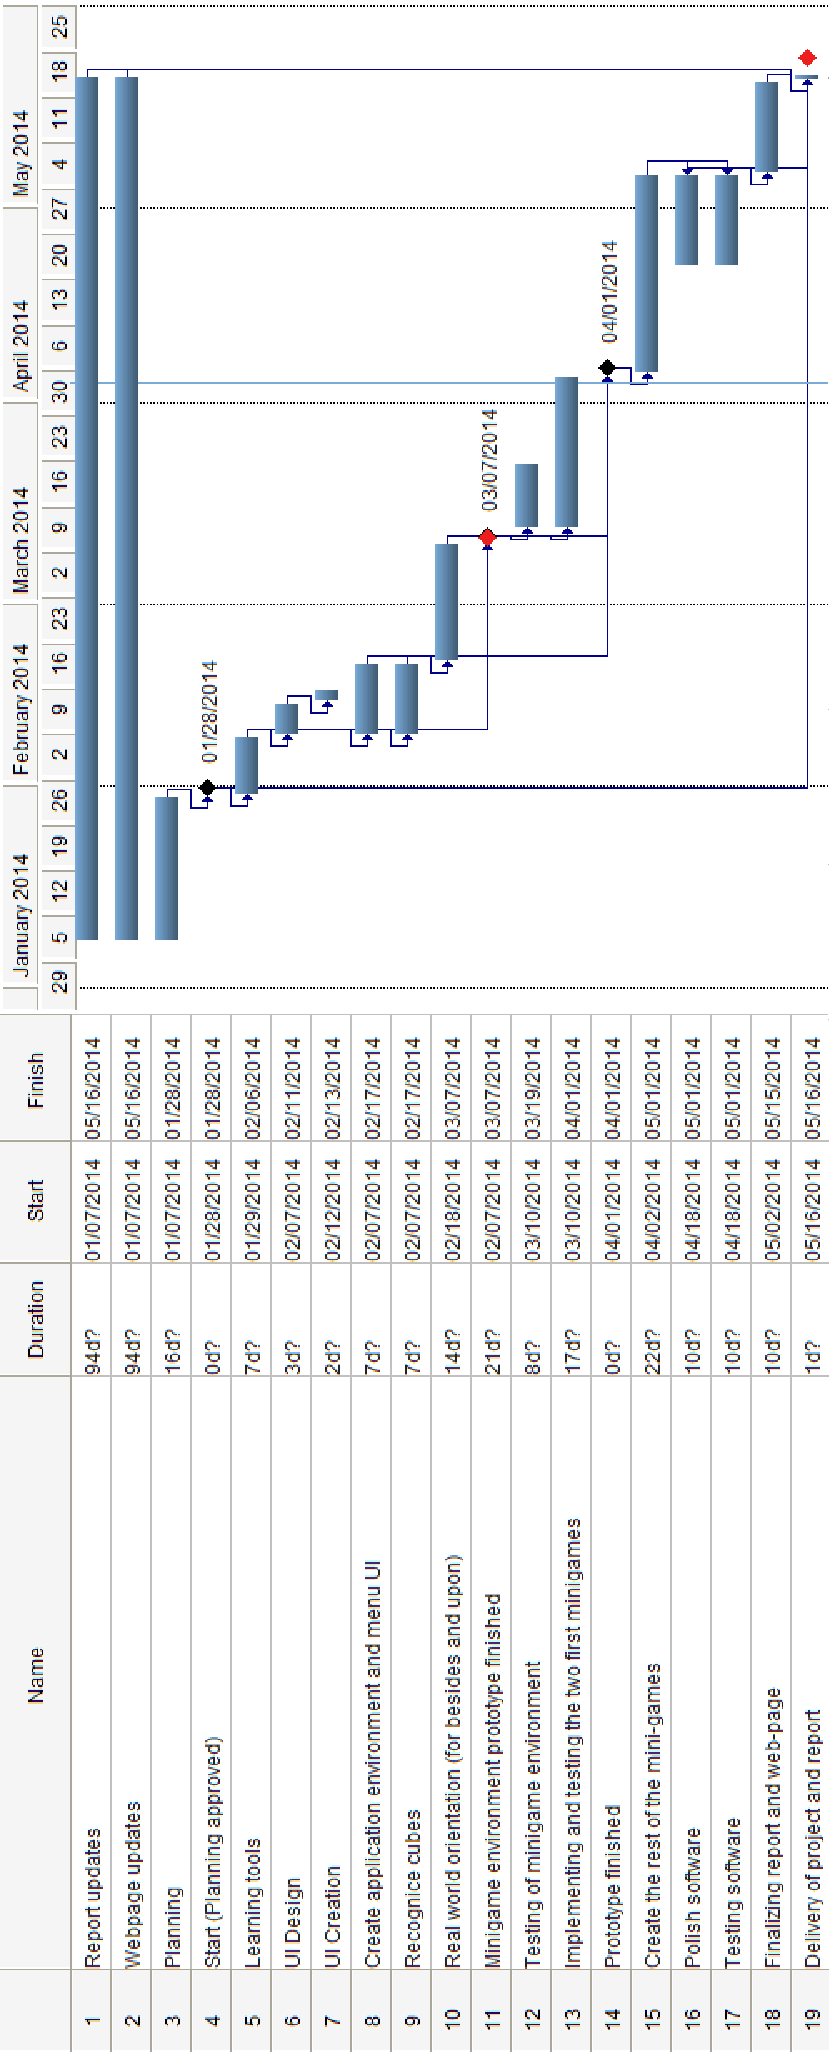
\includegraphics[height=\textwidth, angle=270]{images/preplan_gantt_diagram}
	\caption[Preplan Gantt diagram]{Our initial gantt diagram for the project.}
	\label{fig:preplan_gantt}
\end{figure}


Afterwards we see that the process has been like we have depicted in \autoref{fig:final_gantt}: \nameref{fig:final_gantt}.

\begin{figure}[p]
	\capstart
	\centering

	\begin{ganttchart}[
		hgrid,
		vgrid,
		y unit chart=1.5em,
		bar/.append style={fill=green!60!blue, rounded corners=1pt},
		milestone height=0.7
	  ]{2}{20}
		\gantttitle{Development period}{19} \\
		\gantttitlelist{2,...,20}{1} \\
		% \ganttgroup{Group 1}{1}{7} \\
		\ganttbar{Planning}{2}{6} 
		\ganttbar{}{8}{8} \\

		\ganttbar{Learning Tools}{3}{5} \\

		\ganttbar{Webpage}{5}{6}
		\ganttbar{}{8}{8}
		\ganttbar{}{12}{12}
		\ganttbar{}{14}{14}
		\ganttbar{}{18}{19} \\

		\ganttbar{Final Report}{5}{6}
		\ganttbar{}{12}{12}
		\ganttbar{}{14}{20} \\

		\ganttmilestone{Preplan Delivery}{5} \\

		\ganttgroup{Implementation}{4}{19} \\

		\ganttbar{Prototyping}{4}{6}
		\ganttbar{}{10}{10} \\

		\ganttbar{Gyro}{5}{5} \\

		\ganttbar{Collision Detection}{6}{7} \\

		\ganttbar{Rules}{8}{9}
		\ganttbar{}{11}{11}
		\ganttbar{}{13}{13} \\

		\ganttbar{Grid Feature}{10}{11} \\

		\ganttbar{Pair Feature}{10}{10} \\

		\ganttbar{Chain Feature}{6}{7}
		\ganttbar{}{12}{13} \\

		\ganttbar{Score Screen}{5}{5} \\

		\ganttbar{Register User Screen}{7}{8}\\

		\ganttbar{Loading Screen}{9}{9}
		\ganttbar{}{11}{11}
		\ganttbar{}{13}{13} \\

		\ganttbar{GUI}{6}{7}
		\ganttbar{}{9}{11}
		\ganttbar{}{14}{18} \\

		\ganttbar{Menus}{6}{6}
		\ganttbar{}{14}{14}
		\ganttbar{}{17}{18} \\

		\ganttbar{Level Creator}{8}{13}
		\ganttbar{}{15}{15} \\

		\ganttbar{New Game Script}{12}{12}\\

		\ganttbar{File Loading}{13}{14}\\

		\ganttbar{Logging}{18}{19}\\

		\ganttbar{Testing and Fixing}{14}{14}
		\ganttbar{}{16}{19}\\

		\ganttbar{Code Review}{8}{19}\\


		\ganttbar{GUI}{6}{7}
		\ganttbar{}{9}{11}
		\ganttbar{}{14}{18}\\

		% \ganttbar{Project Setup}{3}{3} \ganttnewline
		% \ganttbar{UI Design}{3}{5} \ganttnewline

		% \ganttbar{Report writing}{14}{20} \\

		% \ganttgroup{Report writing}{14}{20} \\
		\ganttmilestone{Deadline}{20} \ganttnewline

		% \ganttlink{elem1}{elem2}
		% \ganttlink{elem1}{elem3}
		% \ganttlink{elem0}{elem1}
		% \ganttlink{elem2}{elem3}
		% \ganttlink{elem3}{elem4}
	\end{ganttchart}

	\caption[Development Process Gantt Chart]{How the project gantt chart looks like at the end of the development process.}
	\label{fig:final_gantt}

\end{figure}


\subsection{Planning vs reality}%Or how we worked compared to the plan
Our development cycle deviated a lot from the original plan due to a multitude of factors.
For instance we could have allocated less time to the "Create application environment and menu UI" and "Recognice cubes" which each were allocated 7 days in the plan, but had we known more about Unity or the Vuforia plug-in in Unity then we would have known that Unity have methods and functions for creating in-game UI and to make the Vuforia plug-in working were just adding a \gls{prefab} for the camera.
We spent the time allocated to those time slots to creating the framework instead and this additional time shifted a lot of the sub-sequential work a week ahead of time.
Task number 10 (Real world orientation (for besides and upon)) was moved to the beginning of the project by developer Jakob and was done as part of him learning Unity.

The most drastic change in the time schedule is in item 11-15.
After learning some of the inner workings of Unity and how to properly set up a game in Unity it became rapidly apparent that we had taken a somewhat naive approach on it. This was due to our lack of knowledge of how much a game engine can do for us.
Using Unity we had a almost complete mini-game environment from the beginning. As such we only had to program what interaction we wanted to happen when cubes collided.
Our time and efforts were then spent on making the interaction between cubes and the player to what we wanted instead of having to focus on making the basics of a game world working.